\documentclass[conference]{IEEEtran}
\IEEEoverridecommandlockouts
% The preceding line is only needed to identify funding in the first footnote. If that is unneeded, please comment it out.
\usepackage{cite}
\usepackage{amsmath,amssymb,amsfonts}
\usepackage{algorithmic}
\usepackage{graphicx}
\usepackage{textcomp}
\usepackage{xcolor}
\def\BibTeX{{\rm B\kern-.05em{\sc i\kern-.025em b}\kern-.08em
    T\kern-.1667em\lower.7ex\hbox{E}\kern-.125emX}}
\begin{document}

\title{An Enhanced YOLO-based Framework with Deformable Convolutions and Wise-IoU for Pavement Crack Detection in Complex Road Environments\\
{\footnotesize \textsuperscript{*}Note: ...}
\thanks{Identify applicable funding agency here. If none, delete this.}
}

\author{\IEEEauthorblockN{1\textsuperscript{st} Nguyen Pham Minh Triet}
\IEEEauthorblockA{\textit{FPT University HCM} \\
\textit{Ho Chi Minh City}\\
nguyenphamminhtriet2611@gmail.com}
\and
\IEEEauthorblockN{2\textsuperscript{nd} Given Name Surname}
\IEEEauthorblockA{\textit{dept. name of organization (of Aff.)} \\
\textit{name of organization (of Aff.)}\\
City, Country \\
email address or ORCID}
\and
\IEEEauthorblockN{3\textsuperscript{rd} Given Name Surname}
\IEEEauthorblockA{\textit{dept. name of organization (of Aff.)} \\
\textit{name of organization (of Aff.)}\\
City, Country \\
email address or ORCID}
\and
\IEEEauthorblockN{4\textsuperscript{th} Given Name Surname}
\IEEEauthorblockA{\textit{dept. name of organization (of Aff.)} \\
\textit{name of organization (of Aff.)}\\
City, Country \\
email address or ORCID}
\and
\IEEEauthorblockN{5\textsuperscript{th} Given Name Surname}
\IEEEauthorblockA{\textit{dept. name of organization (of Aff.)} \\
\textit{name of organization (of Aff.)}\\
City, Country \\
email address or ORCID}
\and
\IEEEauthorblockN{6\textsuperscript{th} Given Name Surname}
\IEEEauthorblockA{\textit{dept. name of organization (of Aff.)} \\
\textit{name of organization (of Aff.)}\\
City, Country \\
email address or ORCID}
}

\maketitle

\begin{abstract}
This document is a model and instructions for \LaTeX.
This and the IEEEtran.cls file define the components of your paper [title, text, heads, etc.]. *CRITICAL: Do Not Use Symbols, Special Characters, Footnotes, 
or Math in Paper Title or Abstract.
\end{abstract}

\begin{IEEEkeywords}
component, formatting, style, styling, insert
\end{IEEEkeywords}

\section{Introduction}
In an era when traffic is always considered key factor for market development, improving and ensuring transportation infrastructure is a prerequisite for development as well as ensuring public safety is always given top priority.
Therefore, creating an application to assess and detect holes (damaged road sections) or manhole covers on the road is a reasonable solution to help people as well as to help improve and upgrade infrastructure to minimize risks from damaged road sections, helping to improve and ensure safety for people and vehicles participating in traffic. Through the application of image processing methods based on the learning and development ability of Artificial Intelligence. The system will detect and identify, helping to support timely inspection and maintenance through built-in cameras.
The process to build a system includes collecting and labeling each data to pre-processing the data, training the model, evaluating the results, and giving the best and optimal results, when integrating the AI model into the recognition system. Specifically, the development model is based on Computer Vision combined with Deep Learning. The model will use the YOLO object detection model, which will be used as the main basis to identify damaged locations on roads and manhole covers through data collected through cameras image data captured by AI-enabled cameras.
This report focuses on development and construction, as well as providing solutions aimed at improving and ensuring safety for people and vehicles road users and vehicles, mitigating associated risks.


\section{Related Work}
\label{sec:related_work}

\subsection{Traditional Pavement Crack Detection Methods}

Early pavement crack detection methods relied on image processing
techniques such as thresholding, edge detection, morphological
operations, and manually designed texture features. These methods
provide a relatively simple approach to identifying surface
discontinuities, but their performance can be affected by illumination
changes, shadows, surface textures, and irregular crack shapes
\cite{P1_SDNET2018,P8_ConcreteCrackContextAware,P14_PavementCrackDL}.

With the development of deep learning, convolutional neural networks
(CNNs) have enabled automatic feature extraction from pavement images.
Compared with hand-crafted features, CNN-based methods can learn
more representative visual patterns from training data, making them
more suitable for complex road environments
\cite{P11_RDD2020,P13_RoadDamageSurvey,P14_PavementCrackDL}.

\subsection{YOLO-Based Pavement Crack Detection}

YOLO-based object detectors have been widely investigated for road
damage detection because they perform object localization and
classification within a unified detection framework. Different
YOLO-based approaches have explored improvements in feature extraction,
multi-scale representation, and detection efficiency for pavement
cracks and other road defects
\cite{P10_AutomatedPavementCracks,P15_YOLOv5_RoadDamage,
P16_RDD_YOLO,P19_TransXNet_YOLOv8}.

YOLOv8 introduces a detection architecture that supports efficient
feature extraction and multi-scale prediction. Subsequent research
has investigated modified backbones and other architectural
enhancements to improve its performance in crack detection
\cite{P9_ImprovedYOLOv8Concrete,P19_TransXNet_YOLOv8,
P24_YOLOv8_PD,P26_YOLO_DGVG}. More recent detector architectures,
including YOLOv10 and YOLO11, provide additional alternatives for
evaluating the trade-off between detection accuracy and computational
efficiency.

In this study, YOLOv8s, YOLOv10s, and YOLO11s are trained as baseline
models under the same experimental setting. Their results are
compared with those of the proposed YOLOv26n model to investigate
whether the architectural modifications improve pavement crack
detection. The comparison considers detection performance and model
complexity rather than assuming that a newer model necessarily
performs better.

\subsection{Architectural Improvements for Efficient Crack Detection}

Pavement cracks often exhibit thin, elongated, curved, and irregular
shapes. These characteristics create challenges for conventional
convolutional operations, particularly when crack features are weak
or visually similar to background textures. Deformable convolution
addresses this limitation by learning spatial offsets that adapt
feature sampling locations to local geometric patterns
\cite{P20_DeformableConv,P34_InternImage}.

Efficient feature aggregation is another important consideration
for lightweight object detection. GSConv and VoVGSCSP are architectural
components that can be used to construct a more computationally
efficient neck while preserving useful feature information. Their
potential benefits are particularly relevant when detecting small
or thin road defects under limited computational resources
\cite{P26_YOLO_DGVG}.

The detection head also affects model complexity. A shared feature
processing trunk can reduce duplicated computations between
classification and bounding-box regression branches. In the proposed
YOLOv26n architecture, the Grouped Convolution Detection Head (GCH)
is designed to share early feature processing before producing
separate classification and localization predictions.

In addition to architectural changes, bounding-box regression losses
influence localization quality during detector training. Wise-IoU
(WIoU) introduces a dynamic focusing mechanism intended to adjust
the contribution of training samples during bounding-box regression
\cite{P21_WiseIoU}. This provides a relevant research direction for
improving localization, although its effectiveness must be verified
experimentally on the target dataset.

\subsection{Research Gap and Proposed Approach}

Existing research explores different strategies for pavement crack
detection, including modified feature extraction networks, lightweight
architectures, and improved bounding-box regression methods. However,
the effectiveness of these techniques depends on the dataset,
training configuration, and complexity of the target road scenes.

To investigate these issues, this study evaluates four models:
YOLOv8s, YOLOv10s, YOLO11s, and the proposed YOLOv26n. The proposed
model integrates three architectural modifications: C2f-DCNv2 in
the backbone to improve geometric feature representation, GSConv
and VoVGSCSP in the neck to optimize feature aggregation, and a
Grouped Convolution Detection Head (GCH) to reduce duplicated
feature processing.

The objective is to determine whether these modifications provide
a favorable balance between detection accuracy and computational
cost in complex pavement environments. The contribution of each
component should be assessed through experimental comparison and,
where possible, ablation studies.


\section{Method}
The yolov26n (Ours) model combines three core architectural improvements from P26 on the YOLO platform:

\subsection{Backbone: C2f-DCNv2 Module (Crack Geometry Adaptation)}\label{AA}

Regular convolution with a fixed rectangular sampling grid (3x3) struggles to fully capture tiny, twisting cracks. C2f-DCNv2 replaces the second Conv layer in the Bottleneck with Deformable Convolution v2 (DCNv2). DCNv2 automatically learns extra spatial offsets (offsets) of $2K^2$ and modulation masks (mask) of $K^2$ in the [0, 1] range. This allows the receptive field to flex according to the natural shape of cracks D00, D10, D20, while eliminating the influence of background pixels that cause noise.

\subsection{Neck: GSConv and VoVGSCSP (Optimizing Slim-Neck)}

In the neck network, spatial compression operations easily cause the loss of semantic features of small defects. P26 replaces the transitional Conv layers with GSConv (combining Standard Conv and Depthwise Separable Conv 5x5 with Channel Shuffle for inter-channel mixing). At the same time, the entire C2f block in the Neck is replaced with VoVGSCSP following the One-Shot Aggregation (OSA) mechanism, which helps reduce FLOPs and parameters while still maintaining seamless multi-scale information flow.

\subsection{Head: GCH Probe (Grouped Convolution Detection Head)}

The YOLOv8 detection head maintains two independent CBS branches for bounding box (Bbox) and class (Cls), accounting for over 30\% of the total network parameters. GCH merges the first two CBS layers into a shared trunk using Grouped Convolution (g=4 groups), then splits into two Conv2d (1x1) layers to predict coordinates and labels. GCH helps reduce up to 22.28\% of parameters while still ensuring detection accuracy.
\noindent

\textbf{YOLOv26n Architecture Configuration (Ours):}
\begin{itemize}
    \item Backbone: Conv(64, s=2) $\rightarrow$ Conv(128, s=2) $\rightarrow$ C2f\_DCNv2 $\rightarrow$ Conv(256) $\rightarrow$ C2f\_DCNv2 $\rightarrow$ Conv(512) $\rightarrow$ C2f\_DCNv2 $\rightarrow$ Conv(1024) $\rightarrow$ C2f\_DCNv2 $\rightarrow$ SPPF.
    
    \item Neck: FPN + PAN using VGConvSSP (replacing C2f) and GSConv (replacing standard downsampling convolutions).
    
    \item Head: GDetect with multi-scale detection at P3, P4, and P5, using a shared convolutional trunk with 4 groups.
    
    \item Nano (n) scale configuration: \texttt{depth\_multiple: 0.33}, \texttt{width\_multiple: 0.25}. Total number of parameters: 1.89M.
\end{itemize}


\subsection{Experimental Implementation Process}


The team built two complete notebooks to experiment with the \texttt{yolov26n} model in a synchronized manner:

\begin{itemize}[leftmargin=1.5em]
  \item \textbf{Local\_P26.ipynb} (local workstation): Normalizes the data and extracts four classes D00, D10, D20, and D40 (\texttt{rdd2022\_local.yaml}); dynamically registers the P26 modules into Ultralytics; generates \texttt{yolo26n.yaml} and loads the intersection of compatible weights (151 layers) from \texttt{yolov8n.pt}; performs real-time logging and automatic checkpoint resumption.

  \item \textbf{Kaggle\_P26.ipynb} (Kaggle GPU T4/P100): A \textit{self-contained} architecture; leverages the native CUDA backend for all DCNv2 operations; links multi-session checkpoints through \texttt{rdd2022-checkpoints} to safeguard training progress.
\end{itemize}



\section{Results}
    \begin{figure}
        \centering
        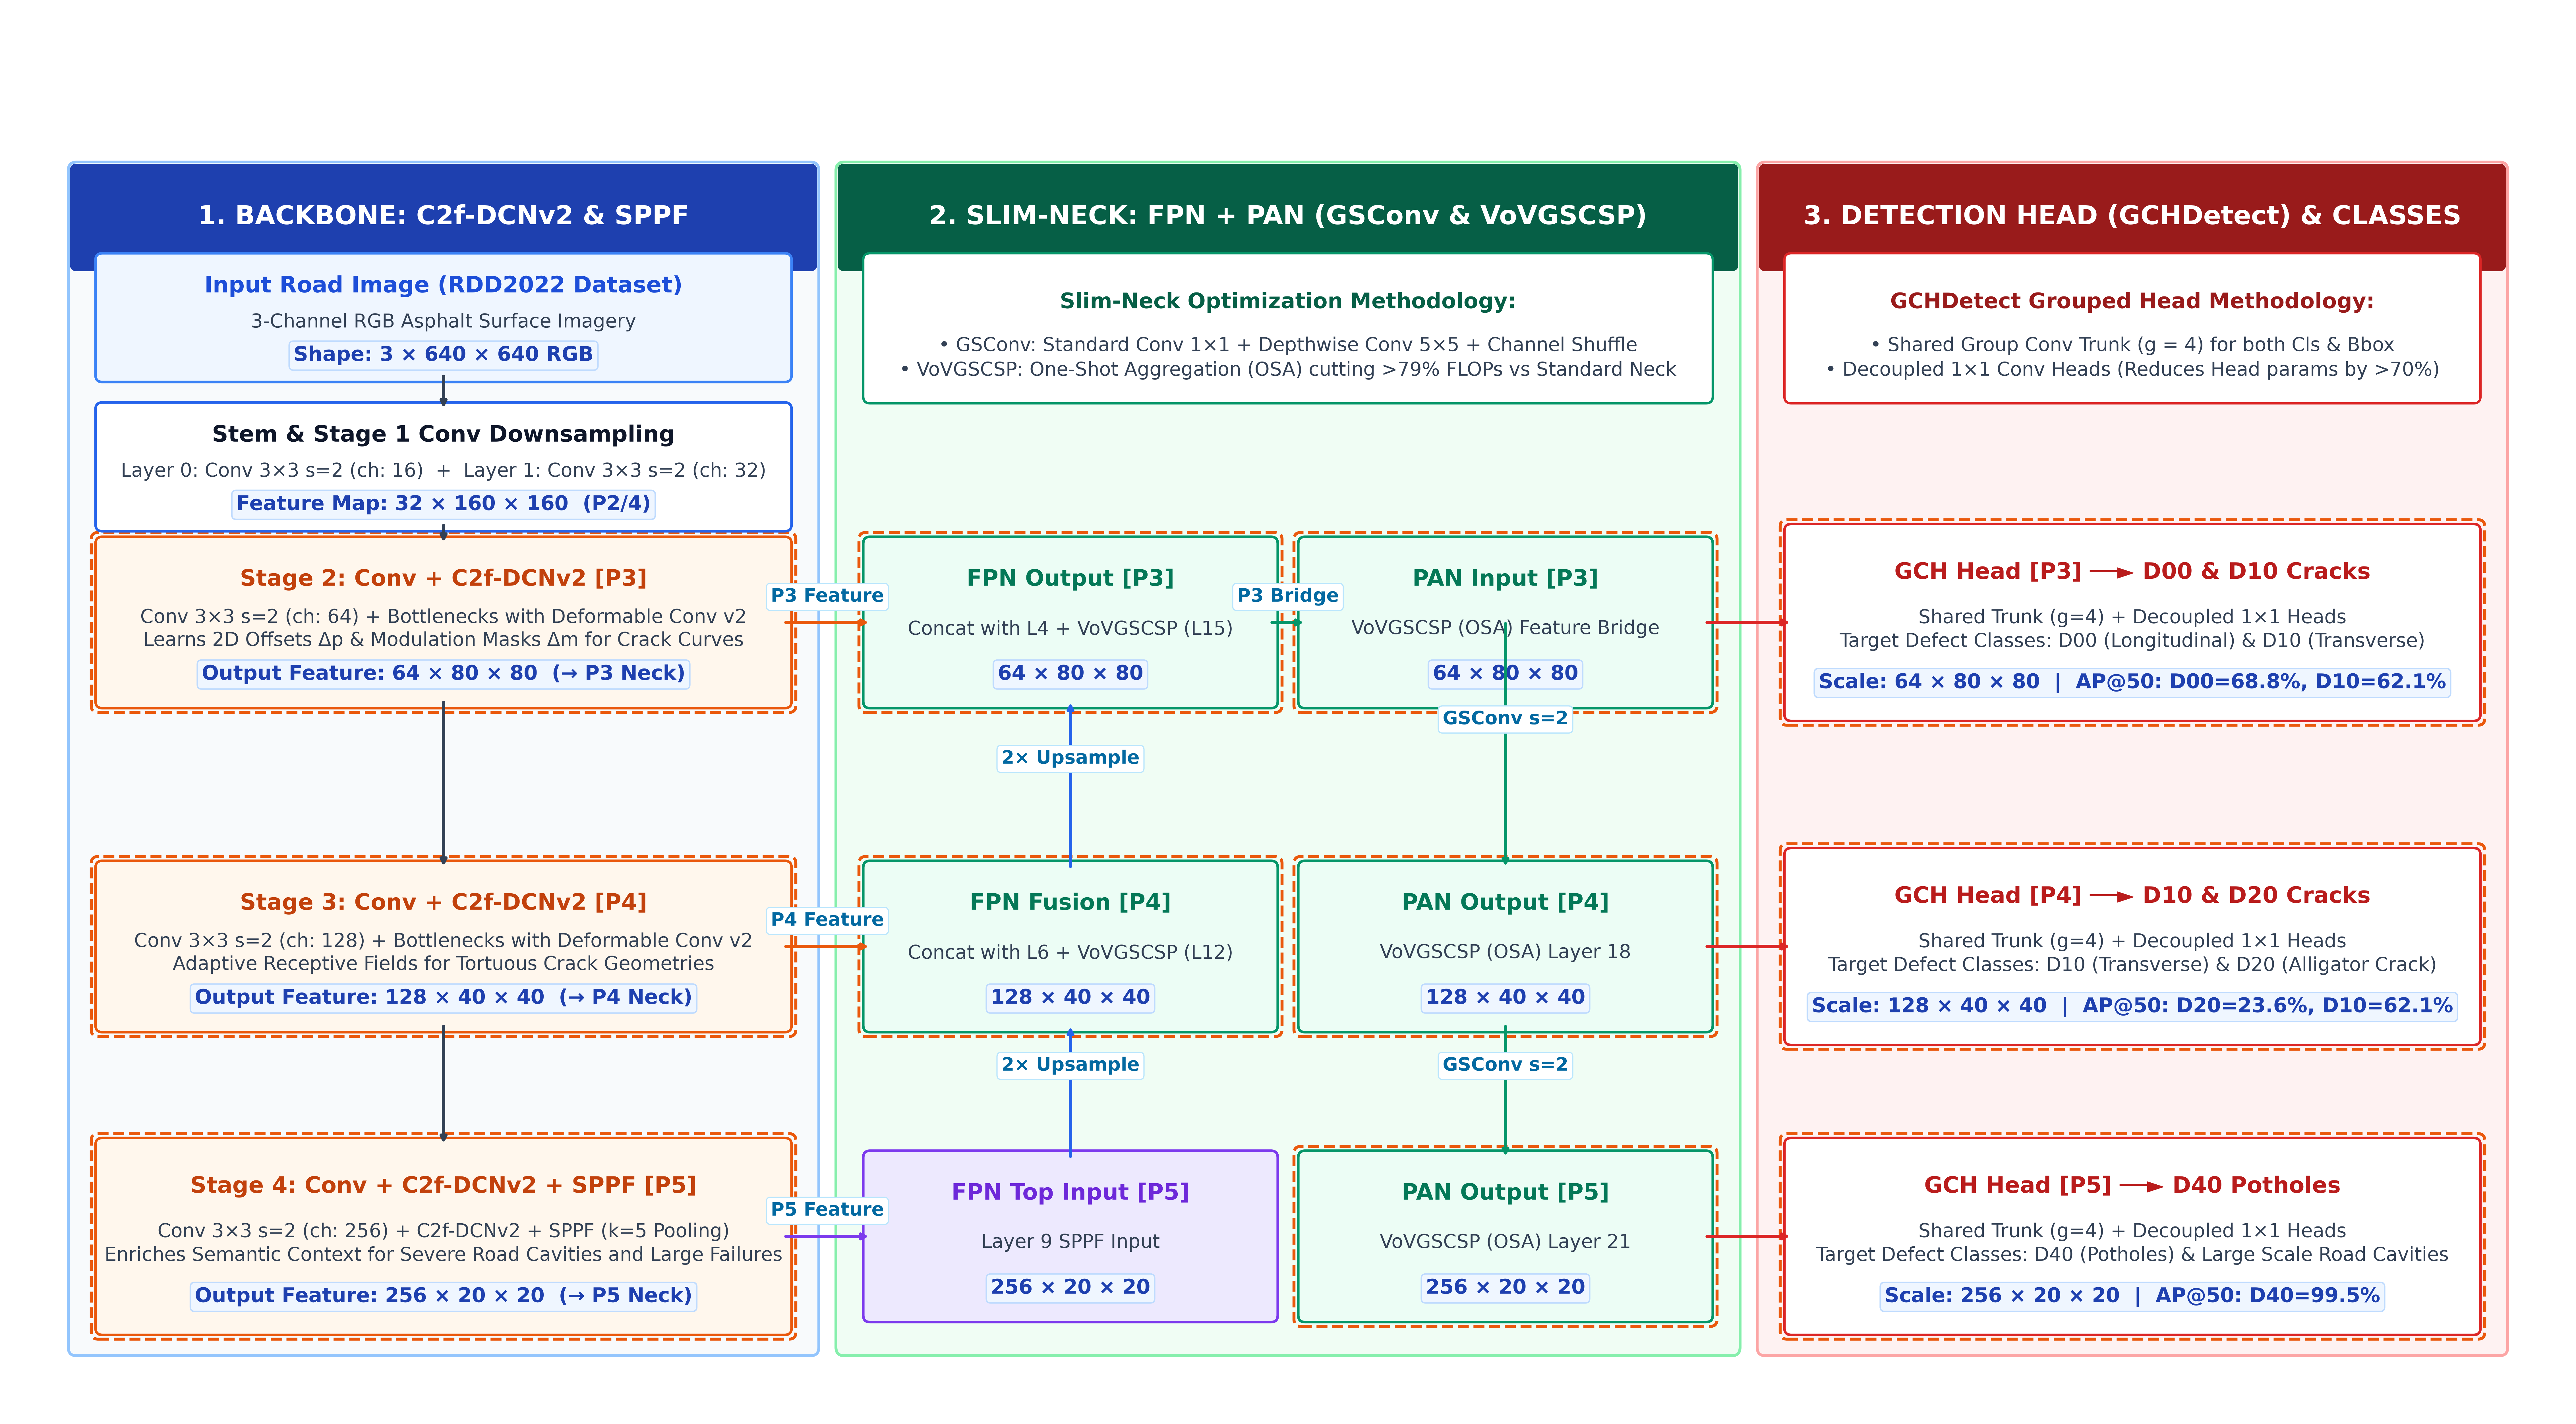
\includegraphics[width=1\linewidth]{f1_architecture_yolov26n.png}
        \caption{Neural Architecture of Yolov26n (Ours)}
        \label{fig:placeholder}
    \end{figure}

\section*{Acknowledgment}

The preferred spelling of the word ``acknowledgment'' in America is without 
an ``e'' after the ``g''. Avoid the stilted expression ``one of us (R. B. 
G.) thanks $\ldots$''. Instead, try ``R. B. G. thanks$\ldots$''. Put sponsor 
acknowledgments in the unnumbered footnote on the first page.

\section*{References}

Please number citations consecutively within brackets \cite{b1}. The 
sentence punctuation follows the bracket \cite{b2}. Refer simply to the reference 
number, as in \cite{b3}---do not use ``Ref. \cite{b3}'' or ``reference \cite{b3}'' except at 
the beginning of a sentence: ``Reference \cite{b3} was the first $\ldots$''

Number footnotes separately in superscripts. Place the actual footnote at 
the bottom of the column in which it was cited. Do not put footnotes in the 
abstract or reference list. Use letters for table footnotes.

Unless there are six authors or more give all authors' names; do not use 
``et al.''. Papers that have not been published, even if they have been 
submitted for publication, should be cited as ``unpublished'' \cite{b4}. Papers 
that have been accepted for publication should be cited as ``in press'' \cite{b5}. 
Capitalize only the first word in a paper title, except for proper nouns and 
element symbols.

For papers published in translation journals, please give the English 
citation first, followed by the original foreign-language citation \cite{b6}.

\begin{thebibliography}{00}
\bibitem{b1} G. Eason, B. Noble, and I. N. Sneddon, ``On certain integrals of Lipschitz-Hankel type involving products of Bessel functions,'' Phil. Trans. Roy. Soc. London, vol. A247, pp. 529--551, April 1955.
\bibitem{b2} J. Clerk Maxwell, A Treatise on Electricity and Magnetism, 3rd ed., vol. 2. Oxford: Clarendon, 1892, pp.68--73.
\bibitem{b3} I. S. Jacobs and C. P. Bean, ``Fine particles, thin films and exchange anisotropy,'' in Magnetism, vol. III, G. T. Rado and H. Suhl, Eds. New York: Academic, 1963, pp. 271--350.
\bibitem{b4} K. Elissa, ``Title of paper if known,'' unpublished.
\bibitem{b5} R. Nicole, ``Title of paper with only first word capitalized,'' J. Name Stand. Abbrev., in press.
\bibitem{b6} Y. Yorozu, M. Hirano, K. Oka, and Y. Tagawa, ``Electron spectroscopy studies on magneto-optical media and plastic substrate interface,'' IEEE Transl. J. Magn. Japan, vol. 2, pp. 740--741, August 1987 [Digests 9th Annual Conf. Magnetics Japan, p. 301, 1982].
\bibitem{b7} M. Young, The Technical Writer's Handbook. Mill Valley, CA: University Science, 1989.
\end{thebibliography}
\vspace{12pt}
\color{red}
IEEE conference templates contain guidance text for composing and formatting conference papers. Please ensure that all template text is removed from your conference paper prior to submission to the conference. Failure to remove the template text from your paper may result in your paper not being published.
\bibliographystyle{IEEEtran}
\bibliography{references}
\end{document}
